\chapter{MARCO TEÓRICO}

\section{MARCO CONCEPTUAL}
\subsection{Goniometría y Análisis vectorial de la mano, antebrazo y muñeca}
La goniometría es la ciencia y técnica que estudia la medición de ángulos, para efectos de este estudio, se medirá la movilidad de las articulaciones mediante un vector que se intercepta en el espacio con otro vector, posteriormente dependiendo del ángulo de esta intersección longitudinal se pude marcar un eje de referencia para así obtener un criterio con respecto a las limitaciones físicas del cuerpo humano \parencite{Taboadela2007TaboadelaLaborales.}

\subsubsection{Goniometría del codo}
El limite de captura del Leap Motion es hasta la muñeca, a partir de una proyección del ángulo de la muñeca se puede determinar la posición del codo debido a la estructura osea y la membrana interosea, este movimiento se denomina pronación y supinación que se da en la muñeca y se producen hasta el codo.\parencite{Taboadela2007TaboadelaLaborales.} 

\begin{figure}[H]
    \centering
    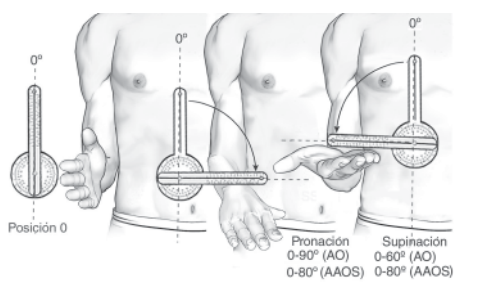
\includegraphics[width=0.5\textwidth]{Anexos/LATEX/chapters/images/pronacion&amp;supinacion.png}
    \caption{pronación y supinación de antebrazo derecho a partir de la posición 0}
    \small{\textbf{Fuente:} \parencite{Taboadela2007TaboadelaLaborales.} }
    \label{GONIOMETRIA_CODO_0}
\end{figure}


Para el correcto análisis es necesario determinar que la posición del paciente, es acostado con el brazo apoyado sobre el decúbito dorsal en posición 0, que el cuerpo quede como si fuera el eje X, y su codo la intersección en 0 del eje Y, se procede a efectuar la flexión y la extensión del codo, donde la extensión pasiva en personas con síndrome de hiperlaxitud\footnote{Patología que genera un alteración en las fibras de colágeno en el tejido conectivo en articulaciones. \parencite[1]{PedroRevistaClinic}} puede ser 0° a 10°(AO) y  Flexión puede ir de 0° - 150°. como se puede observar en la figura 3.

%Asociación para el Estudio de la Osteosíntesis (AO) y la Academia Americana de Cirujanos Ortopédicos (AAOS).

\begin{figure}[H]
    \centering
    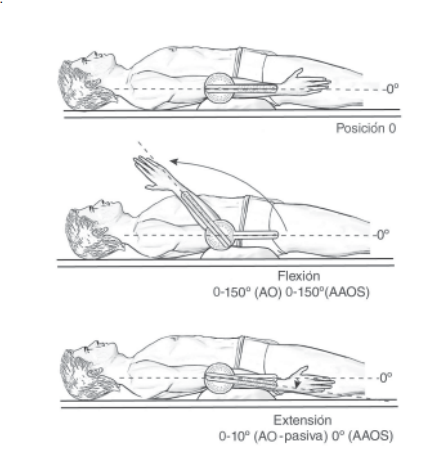
\includegraphics[width=0.6\textwidth]{Anexos/LATEX/chapters/images/goniometria_codo.png}
    \caption{Flexión-extensión del codo derecho a partir de la posición 0}
    \small{\textbf{Fuente:} \parencite{Taboadela2007TaboadelaLaborales.} }
    \label{GONIOMETRIA_CODO}
\end{figure}

\subsubsection{Goniometría del codo Muñeca}
La posición correcta para el análisis en ángulos de la muñeca, es con el paciente sentado con su antebrazo apoyado sobre una mesa, imitando el eje X, y con su punto de intersección sobre el hueso piramidal como eje Y, en está rticulaciín la flexión puede ir en 0 a 50°- 60°(AO) y de 0 a 80° y la extensión de 0 a 35°- 60° (AO) y de 0 a 70° (AAOS).\parencite{Taboadela2007TaboadelaLaborales.}

\begin{figure}[H]
    \centering
    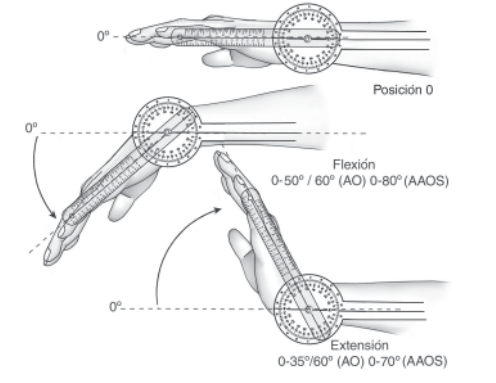
\includegraphics[width=0.6\textwidth]{Anexos/LATEX/chapters/images/goniometria_muneca.png}
    \caption{Flexión-extensión de la muñeca a partir de la posición 0}
    \small{\textbf{Fuente:} \parencite{Taboadela2007TaboadelaLaborales.} }
    \label{GONIOMETRIA_MUNECA}
\end{figure}
%Asociación para el Estudio de la Osteosíntesis (AO) y la Academia Americana de Cirujanos Ortopédicos (AAOS).


\subsubsection{Goniometría del codo Mano}
La posición del paciente debe ser sentado, con el antebrazo totalmente apoyado sobre, rotando 90° el eje X, quedando el punto 0 atravesando imaginariamente el dedo corazón hasta el radio alineado con la linea media del antebrazo, para este movimiento se realiza una desviación radial y una cubital como se puede ilustrar en la figura \ref{GONIOMETRIA_MANO}, donde cada una tiene su correspondiente ángulo, la desviación radial va de 0° a 25°-35° (AO)  y 0° a 20° (AAOS), para la desviación cubital los ángulos van de 0° a 30°-40° (AO) y de 0° a 30° (AAOS).\parencite{Taboadela2007TaboadelaLaborales.}

\begin{figure}[H]
    \centering
    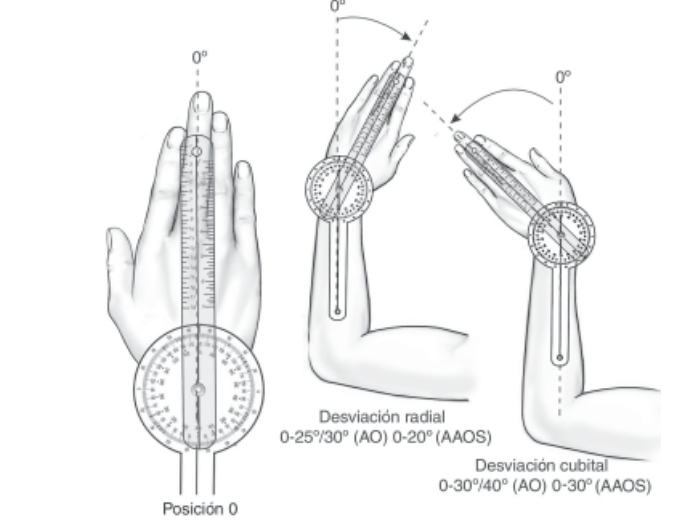
\includegraphics[width=0.6\textwidth]{Anexos/LATEX/chapters/images/goniometria_mano.png}
    \caption{Flexión-extensión de la mano a partir de la posición 0}
    \small{\textbf{Fuente:} \parencite{Taboadela2007TaboadelaLaborales.} }
    \label{GONIOMETRIA_MANO}
\end{figure}


\subsection{Enfermedades y lesiones}
El \parencite{MinisteriodeProteccionSocialdeColombia2006GuiaSuperiores} define un Desorden Músculo Esquelético (DME) como una lesión física originada por trauma acumulado que se desarrolla gradualmente sobre un período de tiempo; como resultado de repetidos esfuerzos\footnote{Se entiende por “esfuerzos repetidos” a un grupo de movimientos continuos mantenidos durante un trabajo que implica la acción conjunta de (..) una parte del cuerpo y provoca en esta misma zona fatiga muscular, sobrecarga, dolor y, por último, lesión.\parencite{INSHT2016PrevencionRepetidos}} sobre una parte específica del sistema músculo esquelético\footnote{Está constituido por los huesos del cuerpo, los músculos, los tendones, los ligamentos, las articulaciones, los cartílagos y otras clases de tejido conjuntivo.}. 

El Instituto Nacional de Seguridad e Higiene en el Trabajo (INSHT) de España ha publicado a lo largo de los años diversas fichas que contienen directrices para la decisión clínica en enfermedades profesionales (DDC) en las cuales se denota una estructura consistente (definición, sintomas, maniobras de exploración, pruebas diagnósticas, vulnerabilidad, actividades de riesgo, repercusión), que posee información completa y depurada acerca de las enfermedades prevalentes en los puestos de trabajo para manos, muñeca y antebrazo.

Considerando lo anterior, se procede a realizar un listado comprensivo de estas enfermedades, tomando como fuente primara de información las fichas expuestas por el INSHT.
 %referencia especialista de salud

\subsubsection{Tenosinovitis De Quervain}
\paragraph{¿Qué es?}
En España, el Instituto Nacional de Seguridad e Higiene en el Trabajo (INSHT) define la Tenosinovitis De Quervainn (TDQ) conocida como tenosinovitis estiloides radiales, como la inflamación de los tendones del pulgar a causa de movimientos repetitivos. \parencite[1]{INSHT2017TendinitisPulgar}

\begin{figure}[H]
    \centering
    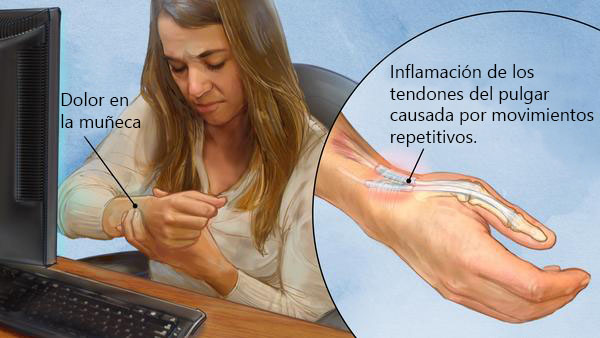
\includegraphics[width=0.7\textwidth]{Anexos/LATEX/chapters/images/TDQ.jpg}
    \caption{Análisis de la mano con Tenosinovitis de Quervain}
    \small{\textbf{Fuente:} https://g.co/kgs/BpkB4A}
    \label{TDQ}
\end{figure}

De acuerdo al \parencite[2]{INSHT2017TendinitisPulgar}, esta enfermedad se manifiesta como una inflamación que produce una estenosis del canal osteofibrososinovial situado en la estiloides radial por el que discurren los tendones del abductor largo y extensor corto del pulgar. Se produce al combinar agarres con giros o desviaciones cubitales y radiales repetidas o forzadas de la mano.
\paragraph{Repercusión}
La Enfermedad de Quervain (CIE-9 MC 727.04)\footnote{CIE-9-MC es un acrónimo de Clasificación Internacional de Enfermedades, Novena Revisión, Modificación Clínica. Se trata de una clasificación de enfermedades y procedimientos utilizada en la codificación de información clínica derivada de la asistencia sanitaria, principalmente en el entorno de hospitales y centros de atención médica especializada.} posee un tiempo estándar de incapacidad transitoria de 20 días.\parencite[6]{INSHT2017TendinitisPulgar}
\paragraph{Prevención}
Se aconseja no combinar agarres con giros o desviaciones cubitales y radiales repetidas. Para las situaciones de oficina que involucran un mouse, es necesario evitar realizar desplazamientos girando la muñeca, el movimiento adecuado debe ser desplazar el brazo en su totalidad desde el hombro. \parencite[5]{INSHT2017TendinitisPulgar}
\subsubsection{Síndrome del Túnel del Carpo}
\paragraph{¿Qué es?}
EL INSHT describe un espacio en la muñeca llamado túnel del carpo, a través del cual pasan el nervio mediano y nueve tendones flexores que van desde el antebrazo hacia la mano\parencite[1]{INSHT2017SindromeCarpiano}. Con base en lo anterior se define el Síndrome del Túnel del Carpo (STC) como una condición producida por la compresión del Nervio Mediano, a nivel de la muñeca. Esta compresión produce entumecimiento, hormigueo y dolor en la mano, dedos y ocasionalmente en el brazo. \parencite[1]{INSHT2017SindromeCarpiano}

\begin{figure}[H]
    \centering
    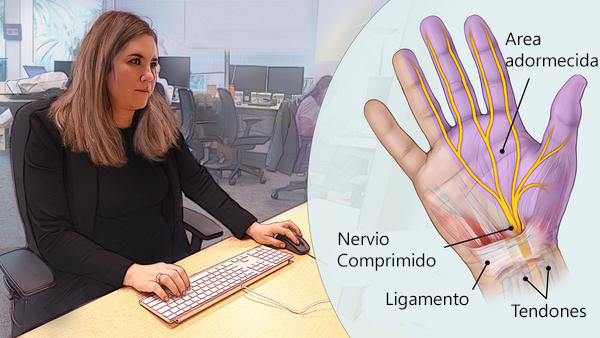
\includegraphics[width=0.7\textwidth]{Anexos/LATEX/chapters/images/STC.jpg}
    \caption{Análisis de la mano con Síndrome del Túnel del Carpo}
    \small{\textbf{Fuente:} https://g.co/kgs/MdPBTe}
    \label{STC}
\end{figure}

Siguiendo la definición dada por el \parencite{INSHT2017SindromeCarpiano}, el STC se presenta cuando se aumenta la presión dentro del túnel por cualquier proceso inflamatorio, comprimiendo el nervio, el cual es una estructura muy sensible a los aumentos de presión. Cuando la presión dentro del túnel es muy alta y altera la función normal del nervio, aparecen rigidez, hormigueo y dolor en la mano y los dedos.
\paragraph{Repercusión}
El Síndrome del Túnel Carpiano (CIE-9 MC 354.0) posee un tiempo estándar de incapacidad transitoria de 60 días\parencite[6]{INSHT2017SindromeCarpiano}.
\paragraph{Prevención}
Para evitar esta enfermedad la \parencite{FundacionSantaFedeBogota2016SindromeTratarlo} recomienda informar al trabajador, entrenándolo para que aquellas posturas o movimientos peligrosos sean evitados durante el desarrollo de su labor, además, el buen diseño de las herramientas, utensilios y del puesto de trabajo ayudan a conseguir la relajación de la mano y de la muñeca.

\subsubsection{Síndrome del túnel cubital}
\paragraph{¿Qué es?}
El \parencite[1]{INSHT2017SindromeCodo} describe esta enfermedad como una mononeuropatía \footnote{Es el daño a un solo nervio que produce pérdida del movimiento, la sensibilidad u otra función de dicho nervio. \parencite{MedlinePlus2018Mononeuropatia}} por compresión del nervio cubital cuando se hace superficial a nivel del codo.
\begin{figure}[H]
    \centering
    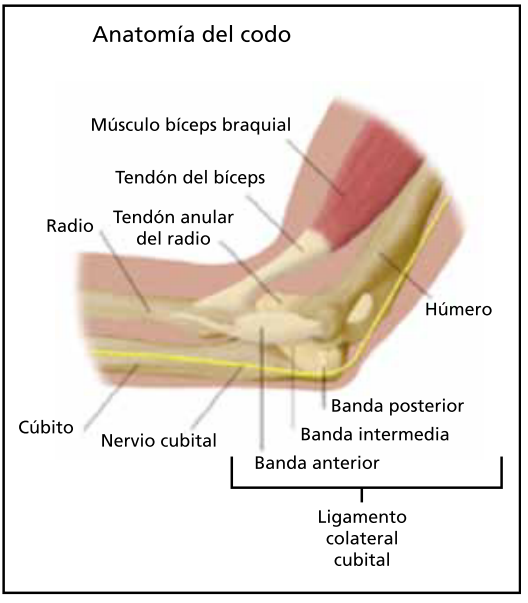
\includegraphics[width=0.4\textwidth]{Anexos/LATEX/chapters/images/AnaCodo.png}
    \caption{Análisis de la mano con Sindrome del túnel cubital}
    \small{\textbf{Fuente:} \parencite[1]{INSHT2017SindromeCodo}}
    \label{AnaCodo}
\end{figure}
\paragraph{Repercusión}
Una lesión del nervio cubital (CIE.9.MC: 352.2) posee un tiempo estándar de incapacidad transitoria de 60 días\parencite[6]{INSHT2017SindromeCodo}.
\paragraph{Prevención}
Evitar trabajos en los que se produzca un apoyo prolongado y repetido de forma directa o indirecta sobre las correderas anatómicas que provocan lesiones nerviosas por compresión, no realizar movimientos extremos de hiperflexión\footnote{Flexión forzada de una extremidad a un grado mayor de lo normal.} y de hiperextensión\footnote{Posición en que se encuentra una articulación al sobrepasar su posición anatómica neutral.} del codo.\parencite[5]{INSHT2017SindromeCodo}.


\section{MARCO REFERENCIAL}
\subsection{Modelos de valoración de riesgos posturales en Colombia}
\subsubsection{Normas GATI-SO}
Las Guías de Atención Integral de Salud Ocupacional Basadas en la Evidencia (GATI-SO) nacen a partir de un plan de trabajo propuesto por la dirección general de riesgos profesionales del ministerio de la protección social Colombiano con el objetivo de incrementar el diagnóstico y prevenir las enfermedades profesionales de
mayor prevalencia en Colombia \parencite[6]{MinisteriodeProteccionSocialdeColombia2006GuiaSuperiores}, esto se lleva a cabo a partir de la emisión de recomendaciones basadas en la evidencia.

Las características de los factores de riesgo ocupacional que han demostrado estar asociados con la aparición del \textbf{STC} son las siguientes:\parencite[45]{MinisteriodeProteccionSocialdeColombia2006GuiaSuperiores}
\begin{itemize}
\item Posturas en flexión y extensión de dedos, mano y muñeca, así como, la desviación ulnar o radial que implique agarre, pronación y supinación combinada con el movimiento repetitivo en ciclos de trabajo
\item Fuerza ejercida en trabajo dinámico por manipulación de pesos en extensión y flexión de los dedos y la mano
\item Vibración segmentaría derivada del uso de herramientas vibratorias
\end{itemize}
Las características de los factores de riesgo ocupacional que han demostrado estar asociados con la aparición del \textbf{TDQ} son las siguientes\parencite[45]{MinisteriodeProteccionSocialdeColombia2006GuiaSuperiores}:
\begin{itemize}
\item Postura forzada de muñeca asociada a movimiento de alta repetición (ciclos de tiempo menores a 30 segundos o 50 \% del ciclo gastado.
\end{itemize}
Adicionalmente se mencionan las siguientes conclusiones \parencite[46]{MinisteriodeProteccionSocialdeColombia2006GuiaSuperiores}:
\begin{itemize}
\item Existe evidencia de que las posturas asumidas de codo, antebrazo y mano se asocian con mayor frecuencia a los desórdenes de trauma acumulativo en población trabajadora.
\item Existe evidencia de que el movimiento repetitivo se asocia con mayor frecuencia a los desórdenes de trauma acumulativo en población trabajadora.
\item Existe evidencia de que la fuerza se asocia con mayor frecuencia a los desórdenes de trauma acumulativo en población trabajadora.
\end{itemize}
\subsection{Modelos de valoración de riesgos posturales internacionales}
A lo largo de los años se han consolidado diversas metodologías para realizar análisis de los factores de riesgo presentes en los puestos de trabajo, estas herramientas han sido estudiadas, consolidadas y depuradas por algunas entidades especializadas en la ergonomía en el trabajo. En la Universidad Politécnica de Valencia el grupo de investigación de ergonomía en el trabajo y prevención de riesgos laborales, conocido como Ergonautas (Dirigido por Phd. José Antonio Diego-Más), presenta un compendio de información que recopila todos los temas necesarios para realizar una correcta evaluación del puesto de trabajo. En cuanto a la evaluación de posturas, esta plataforma comprende una estructura estándar que facilita el entendimiento, la legibilidad y además proporciona una descripción enriquecida de los métodos tradicionales con bibliografía complementaria. 

Con base en lo anterior, Ergonautas representa una herramienta de apoyo útil para los objetivos de esta investigación, consolidándose como una de las fuentes primarias de información para las secciones presentadas a continuación.

\subsection{Método Rula}
El método RULA \textit{(Rapid Upper Limb Assessment)} tiene como objetivo de evaluar la exposición de los trabajadores a factores de riesgo que originan una elevada carga postural\footnote{Llevar a cabo posturas inadecuadas a manera continua o repetitiva que generen fatiga} y que pueden ocasionar trastornos en los miembros superiores del cuerpo. Para la evaluación del riesgo se consideran el método la postura adoptada, la duración, la frecuencia y las fuerzas ejercidas cuando se mantiene.\parencite[2]{Mcatamney1993RULA:Disorders}

El método RULA evalúa una determinada postura y esta obtiene una puntuación con base a los ángulos generados, estableciendo así un denomiando \textit{Nivel de Actuación}. El Nivel de Actuación indicará si la postura es aceptable o en qué medida son necesarios cambios o rediseños en el puesto. En resumen, RULA permite al evaluador detectar posibles problemas ergonómicos derivados de una excesiva carga postural.\parencite{Diego-Mas2015EvaluacionRULA}\parencite[4]{Mcatamney1993RULA:Disorders}

\parencite{Diego-Mas2015EvaluacionRULA} indica que RULA divide el cuerpo en dos grupos, el Grupo A que incluye los miembros superiores (brazos, antebrazos y muñecas) y el Grupo B, que comprende las piernas, el tronco y el cuello. Mediante las tablas asociadas al método, se asigna una puntuación a cada zona corporal (piernas, muñecas, brazos, tronco, etc.) para, en función de dichas puntuaciones, asignar valores globales a cada uno de los grupos A y B.
\subsection{Método Reba}
REBA \textit{(Rapid Entire Body Assessment)} es un método basado en el previamente mencionado método RULA, diferenciándose fundamentalmente en la inclusión en la evaluación de las extremidades inferiores. Según \parencite{Diego-Mas2015EvaluacionREBA} REBA es uno de los métodos observacionales para la evaluación de posturas más extendido en la práctica.

Según expone \parencite{Hignett2000RapidREBA} REBA es un método de análisis postural acondicionado para evaluar las tareas que poseen cambios repentinos de postura, generalmente a causa de la manipulación de cargas inestables o impredecibles. Este método ayuda al evaluador a identificar los posibles riesgos relacionados a una postura, principalmente de tipo músculo-esquelético, orientando en cada circunstancia la inmediatez con la que se tienen que efectuar acciones correctivas.

\parencite{Diego-Mas2015EvaluacionREBA} resalta que el método REBA evalúa posturas individuales y no conjuntos o secuencias de posturas, por ello, recomienda seleccionar aquellas posturas que serán evaluadas de entre las que adopta el trabajador en el puesto. Luego, seleccionar aquellas que, a priori, supongan una mayor carga postural bien por su duración, bien por su frecuencia o porque presentan mayor desviación respecto a la posición neutra.
\subsection{Método Owas}
OWAS \textit{(Ovako Working Posture Analysing System)} es un sistema de evaluación de posturas de trabajo que analiza todas las posturas realizadas por el trabajador a lo largo de su jornada, con la ventaja de evaluar el riesgo de todas las posturas adoptadas de manera conjunta con base en la frecuencia y la gravedad.\parencite{MattilaMVilkki1999OccupationalSystems}

Este método es observacional, es decir, parte de la observación de las diferentes posturas adoptadas por el trabajador durante el desarrollo de la tarea a intervalos regulares \parencite{Diego-Mas2015EvaluacionOWAS}. Las posturas distinguidas son clasificadas en 252 posibles combinaciones dada la posición de los brazos, la espalda, y las piernas del trabajador, además, considera el peso con el que se realiza el movimiento. 

El autor citado anteriormente observó que como contrapartida, OWAS suministra estimaciones menos exactas, sin embargo, es la habilidad de contemplar un conjunto de posturas a través de la jornada laboral lo que consigue que OWAS siga siendo un método relevante a través de los años y continúe como uno de los más empleados en la evaluación de la carga postural.
\subsection{Método Ergo/IBV}
El método ERGO/IBV permite analizar tareas repetitivas de miembro superior con ciclos de trabajo claramente definidos, con el fin de evaluar el riesgo de lesión musculo esquelética en la zona del cuello-hombro y en la zona de la mano-muñeca.\parencite{Nogareda2009TareasErgonomicos}.

Para realizar una evaluación se requiere observar las posturas adoptadas por el trabajador, asignándoles un porcentaje que represente la cantidad de tiempo que ocupa esa actividad sobre el total, luego, se puntúa cada postura con respecto a el grado de inclinación desde la posición natural y finalmente se multiplica para ponderar el factor de riesgo.\parencite{Nogareda2009TareasErgonomicos}.
\section{MARCO TECNOLÓGICO}
\subsection{Inteligencia Artificial}
\subsubsection{Aprendizaje de máquina}
Conocido también como Machine Learning (ML) es definido de manera general por \parencite{MehryarMohriAfshinRostamizadeh2012FoundationsLearning} como "Métodos computacionales usando experiencia para mejorar el desempeño o hacer predicciones precisas". Para \parencite{Flach2012MachineLearning} "es el estudio sistemático de algoritmos y sistemas
que mejoran su conocimiento o desempeño con experiencia". Para ambos casos la "experiencia" se refiere a la información disponible para el aprendiz, la cual generalmente se encuentra en la forma de información electrónica recopilada y puesta a disposición para análisis.

Los algoritmos de aprendizaje de máquina han sido implementados satisfactoriamente en múltiples áreas como la clásificación de texto, procesamiento de lenguaje natural, reconocimiento de voz, reconocimiento óptico de caracteres (OCR), visión artificial, detección de fraude, videojuegos, control asistido de vehículos, diagnósticos médicos, sistemas de recomendación y otras más.\parencite{MehryarMohriAfshinRostamizadeh2012FoundationsLearning}.

Tales aplicaciones responden a una serie de problemas de aprendizaje, según \parencite{MehryarMohriAfshinRostamizadeh2012FoundationsLearning} algunas de las categorías principales son:
\begin{itemize}
    \item Clasificación: Asignar una categoría a cada objeto
    \item Regresión: Predecir un valor real para cada objeto
    \item Ranking: Ordenar objetos de acuerdo a cierto criterio
    \item Agrupamiento (Clustering): Particionar objetos en regiones homogéneas
    \item Reducción de la dimensionalidad no lineal (Manifold learning): Transformar una representación inicial de objetos, hacia una representación con menores dimensiones preservando las propiedades iniciales
\end{itemize}

Es importante resaltar que la exactitud del clasificador empleado se encuentra estrictamente relacionado con el proceso de entrenamiento y el clasificador utilizado, adicionalmente, la elección de los parámetros es fundamental para que el aprendizaje sea exitoso. \parencite[7]{Flach2012MachineLearning}

Dicho lo anterior, es imperativo revisar cómo opera cada uno de estos clasificadores.
\paragraph{Árboles de Decisión (AD)}
Un árbol de decisión representa una función que toma como entrada un vector de valores de atributo y devuelve una "decisión": un único valor de salida. La inducción de árboles de decisión es una de las formas más simples y exitosas de aprendizaje de máquina.\parencite[697]{Russel2010Artificial_Intelligence_3rd}.

Los arboles de decisión realizan una serie de valoraciones sobre los atributos de entrada $A_i$ al pasar por cada nodo, y las ramas poseen etiquetas con los posibles valores del atributo, $A_i = V_{ik}$

\begin{figure}[H]
    \centering
    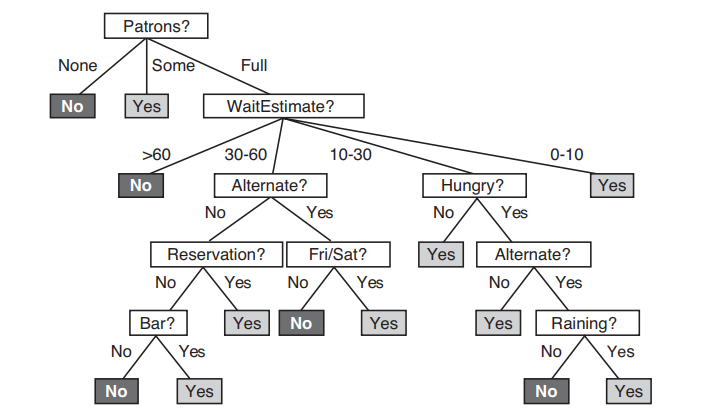
\includegraphics[width=1\textwidth]{Anexos/LATEX/chapters/images/add.PNG}
    \caption{Árbol de decisión para decidir si esperar una mesa}
    \small{\textbf{Fuente:} \parencite[699]{Russel2010Artificial_Intelligence_3rd}}
    \label{add}
\end{figure}

Una de las maneras para poder obtener una división óptima de los datos es realizar un cálculo de entropía\footnote{Para \parencite[703]{Russel2010Artificial_Intelligence_3rd} la entropía \textit{“Es una medida de incertidumbre para una variable
aleatoria; la adquisición de información corresponde a la reducción en la entropía.”}} sobre el vector de entrada. El objetivo es buscar la variable que aporte la mayor cantidad de información (entropía menor), aquellas con esta cualidad tienen más probabilidad de ser elegidas como nodos principales.

\paragraph{Redes Neuronales Artificiales (ANN)}
Uno de los pilares de la neurociencia es que la actividad mental consiste principalmente de electroquímica entre redes de celulas cerebrales llamadas neuronas. Inspirados por esta hipótesis, algunos de los primeros desarrollos de IA fueron orientados a crear redes neuronales artificiales. \parencite[727]{Russel2010Artificial_Intelligence_3rd}

\begin{figure}[H]
    \centering
    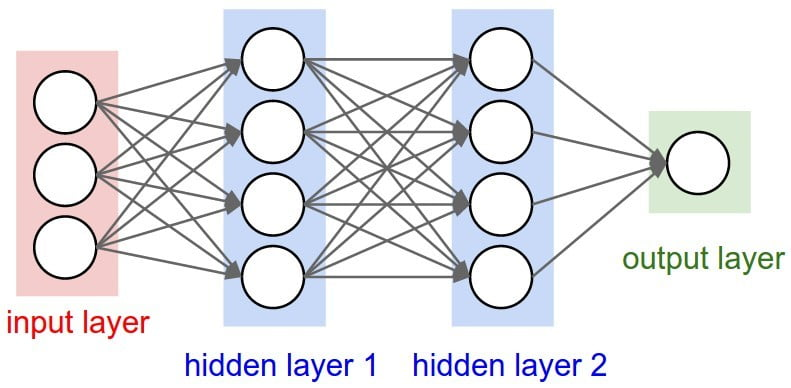
\includegraphics[width=0.7\textwidth]{Anexos/LATEX/chapters/images/ann.jpg}
    \caption{Esqueleto de una red neuronal artificial}
    \small{\textbf{Fuente:} IBM Knowledge Center}
    \label{ann}
\end{figure}

A grandes rasgos, los componentes de una neurona son: Entradas, función de entrada, función de activación, salida y enlaces de salida. Las propiedades de la red son determinadas por su topología y algunas características de sus neuronas, sin embargo, el funcionamiento es el mismo, una neurona se "dispara" cuando una combinación lineal de entradas supera cierto limite.
\paragraph{Máquinas de Soporte Vectorial (SVM)}
\subsection{Sensores Ópticos}
\subsubsection{Leap Motion}
Leap Motion es un sensor óptico que realiza el seguimiento de gestos y posiciones para la manos sin necesidad de hacer contacto con el dispositivo. Consta de de tres pulgadas de largo y una de ancho. Equipado con tres emisores infrarrojos y dos cámaras infrarrojas es capaz de reportar movimientos con precisión submilimétrica. \parencite{Weichert2013AnalysisController.}

\begin{figure}[H]
    \centering
    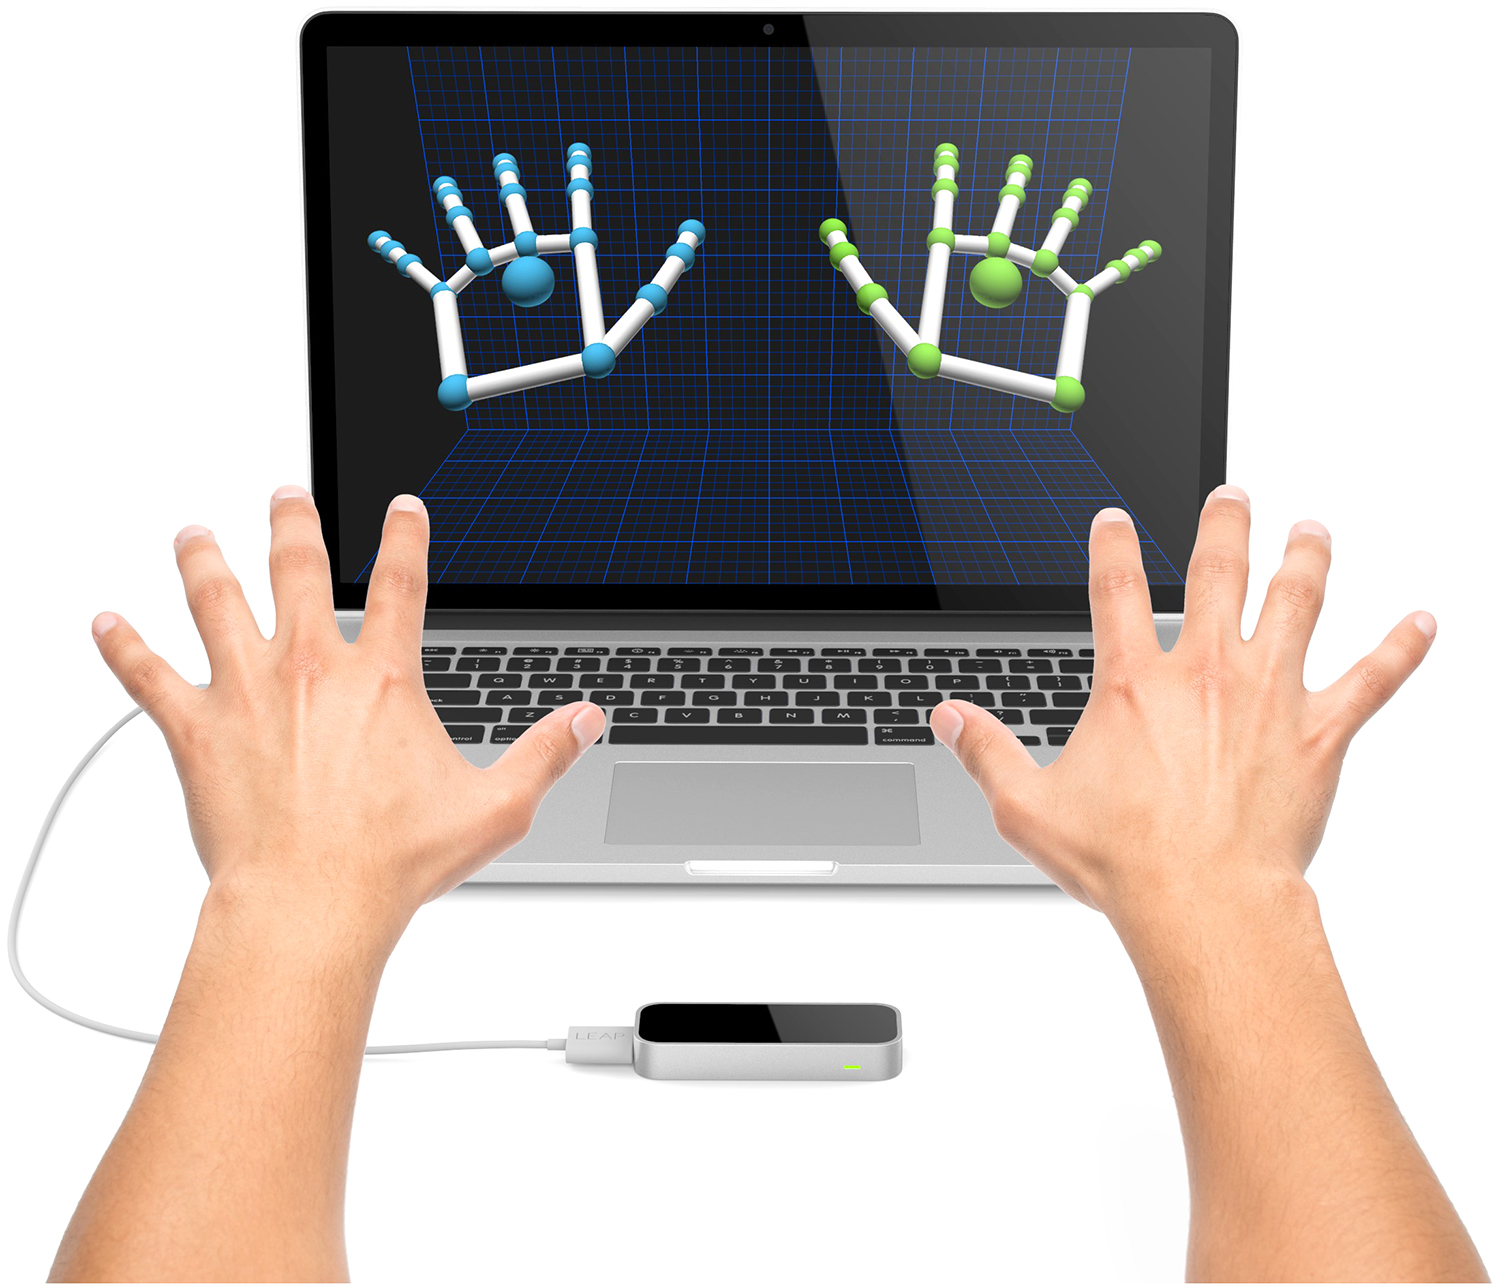
\includegraphics[width=0.5\textwidth]{Anexos/LATEX/chapters/images/leapmotion.jpg}
    \caption{Dispositivo Leap Motion y su renderizado}
    \small{\textbf{Fuente:} Leap Motion | Leapmotion.com}
    \label{LeapOverview}
\end{figure}

El rango de captura de movimientos va desde el antebrazo hasta la punta de los dedos, esto permite reconocer posturas muy precisas de los miembros distales superiores en coordenadas relativas al sensor en un plano (X,Y,Z), haciendo uso de su sistema estereoscópico\footnote{Técnica para crear o mejorar la ilusión de profundidad en una imagen mediante estereopsis para visión binocular.} a cabalidad.

Su uso está preparado para funcionar y fusionarse facilmente con el framework Unity, esta herramienta se puede implementar en otros proyectos desligados de este framework\parencite{LeapMotionInc.2018LeapDeveloper}
\subsection{Motor de Desarrollo}
\subsubsection{Unity}
Unity es un motor de juegos multiplataforma desarrollado por Unity Technologies que funciona mediante un editor visual y scripting\footnote{Codificar una serie de instrucciones que son ejecutadas por un programa de computador.} en C\#, puede ser usado para crear tanto juegos bidimensionales y tridimensionales como simulaciones para sus múltiples plataformas. Contando con una licencia gratuita y tres opciones de licencia paga, esta plataforma se ha convertido en el software de motor de juegos \#1 en el 2018, destacado por su facilidad de uso y satisfacción del cliente.\parencite{G2Crowd2018Best2018}

Desde sus orígenes Unity se ha caracterizado por ofrecer las herramientas necesarias para realizar desarrollos de X Reality (XR)\footnote{Abarca un amplio espectro de hardware y software, incluidas las interfaces sensoriales, las aplicaciones y las infraestructuras, que permiten la creación de contenido para realidad virtual (VR), realidad mixta (MR), realidad aumentada (AR), realidad cinematográfica (CR).}, ofreciendo una gran compatibilidad con múltiples dispositivos de hardware de esta misma categoría. Algunas de las ventajas de utilizar Unity sobre otro motor, son:
\begin{itemize}
    \item \textbf{Desarrollo multiplataforma}: Unity cuenta con soporte extendido a 25 plataformas.\parencite{UnityTechnologies2018UnityPlatforms} La aplicación desarrollada y desplegada se puede compartir fácilmente entre PC, web y plataformas móviles. 
    \item \textbf{Metodología ágil}: Permite la creación rápida de prototipos y los lanzamientos constantes, que a su vez aceleran el desarrollo del juego.
    \item \textbf{Documentación}: La documentación de la plataforma es fácil y muy detallada, incluye la explicación de cada tema sin importar lo pequeño que sea.
    
\end{itemize}
    
\subsection{Metodología ingeniería de software}
\subsubsection{SCRUM}

En el año 1996 por Ken Schwaber y Jeff Sutherland nace esta metodología basada en la formación más reconocible de rugby, en la que ambos equipos se empujan entre si para obtener el balón y sacarlo de la formación sin tocarlo con la mano, la cual posee este mismo nombre, SCRUM \parencite{AlexanderMenzinskyGertrudisLopez2016ScrumManage}, busca aprovechar las características de un equipo y enfocarlas a evitar retrasos  e ir ajustando en diferentes partes del proceso de forma iterativa, este permite una rápida toma de decisiones frente a las eventualidades en el desarrollo.


Esta metodología se puede utilizar en todo tipo de desarrollo de software, desde desarrollar paquetes de software completos o solo algunas partes de sistemas más grandes, teniendo en cuenta que es importante que en estos proyectos quienes los ejecutan tengan en cuenta los pilares de auto-organización y la comunicación dentro del equipo,en general solo se definen con algunas reglas, roles, artefactos y eventos, pero cada uno de estos elementos tiene un propósito especifico y esencial.

los componentes principales de SCRUM están definidos por 
\begin{itemize}
    \item Tres roles: Scrum Master, el propietario del producto (Product Owner) y el equipo desarrollo
    \item Un Backlog priorizado que contiene los requisito del usuario final.
    \item Sprints o iteraciones
    \item Eventos Scrum: En estos se encuentran, la reunión de planificación de Sprint(QUÉ-reunión, HOW-Meeting), reunión diaria de Scrum, reunión de revisión de Sprint, Sprint retrospective meeting 
\end{itemize}

para entender el proceso de Scrum es necesario abordar cada uno de estos elementos ,a continuación se realiza una descripción general, de lo establecido por la metodología. 

\paragraph{Roles}
Los roles en Scrum se dividen en personas comprometidas con el proyecto y personas que se benefician del proyecto, para las personas comprometidas con el proyecto se encuentran
\begin{itemize}
    \item Product Owner, Este es como se traduce el propietario del producto, persona que toma las decisiones y conoce el negocio del cliente junto la visión que este tiene acerca del producto final, se encarga de reunirse con el cliente, tomar las ideas y ordenarlas por prioridad en el Product Backlog
     \item Scrum Master, Comprueba que el modelo y metodología funcionan , está encargado de eliminar los inconvenientes que hagan interrumpir el proceso, también interactúa con el cliente.
     \item Equipo desarrollo, El tamaño del equipo depende de el tipo de solución a desarrollar, tienen autoridad para organizarse y tomar decisiones con el foco puesto en el objetivo, está 100\% involucrado con la estimación del esfuerzo en as tareas de Product Backlog.
\end{itemize}

Por otra parte, se encuentran las personas que se benefician con el proyecto, que aunque no son parte del proceso de SCRUM, es necesaria su información para la retroalimentación de la salida y así poder verificar,revisar y planear cada uno de los Sprints.
\begin{itemize}
    \item Usuarios, Es el destinatario del producto final. 
    \item Stakeholders, personas que se benefician de cada revisión de Sprint
    \item Managers, Toma las decisiones participando en la selección o filtro de objetivos y requisitos. 
\end{itemize}

\paragraph{Artefactos}

\begin{itemize}
    \item Pila del producto (Product backlog), Está conformada por la lista de requerimientos del usuario, que a partir de la visión del producto va creciendo y evolucionando durante el proceso de desarrollo.
    \item Pila del sprint(Sprint backlog), Esta es la lista de trabajos y tareas que debe realizar el equipo de desarrollo para generar el incremento meta. 
    \item Incremento, es el resultado de cada iteración (Sprint)
\end{itemize}


\paragraph{Eventos}